This section will describe, at different levels of abstraction, the architecture of \projectname~system. We will use: component diagrams to show the structure of the various software components and their interactions in the form of interfaces; deployment diagrams to show how the software artifacts will be arranged in the various physical devices; sequence diagrams to give a deeper representation of the information flow between the various components and subsystems. At the end we will also provide a table to show how every requirement listed in the RASD document will be mapped to one or more software components. \\
\projectname~architecture will be structured around two main divisions:
\begin{itemize}
\item \textbf{Client Side/Server Side}: the first one will be located on the users' physical device, such as computers and smartphones, while the second one will be deployed in a hosted server; the main logic of the system will be run server side. With our architecture different clients will be supported with the same server application.
\item \textbf{Internal Components/External Components}: the first ones will be implemented by our development team or purchased on the marked as standalone components and will be the core of the system, while the second ones will be operated through interfaced over the internet protocol. We will use external components whenever they will have better features and lower costs than the ones that we could develop internally.
\end{itemize}

\begin{figure}[h]
	\centering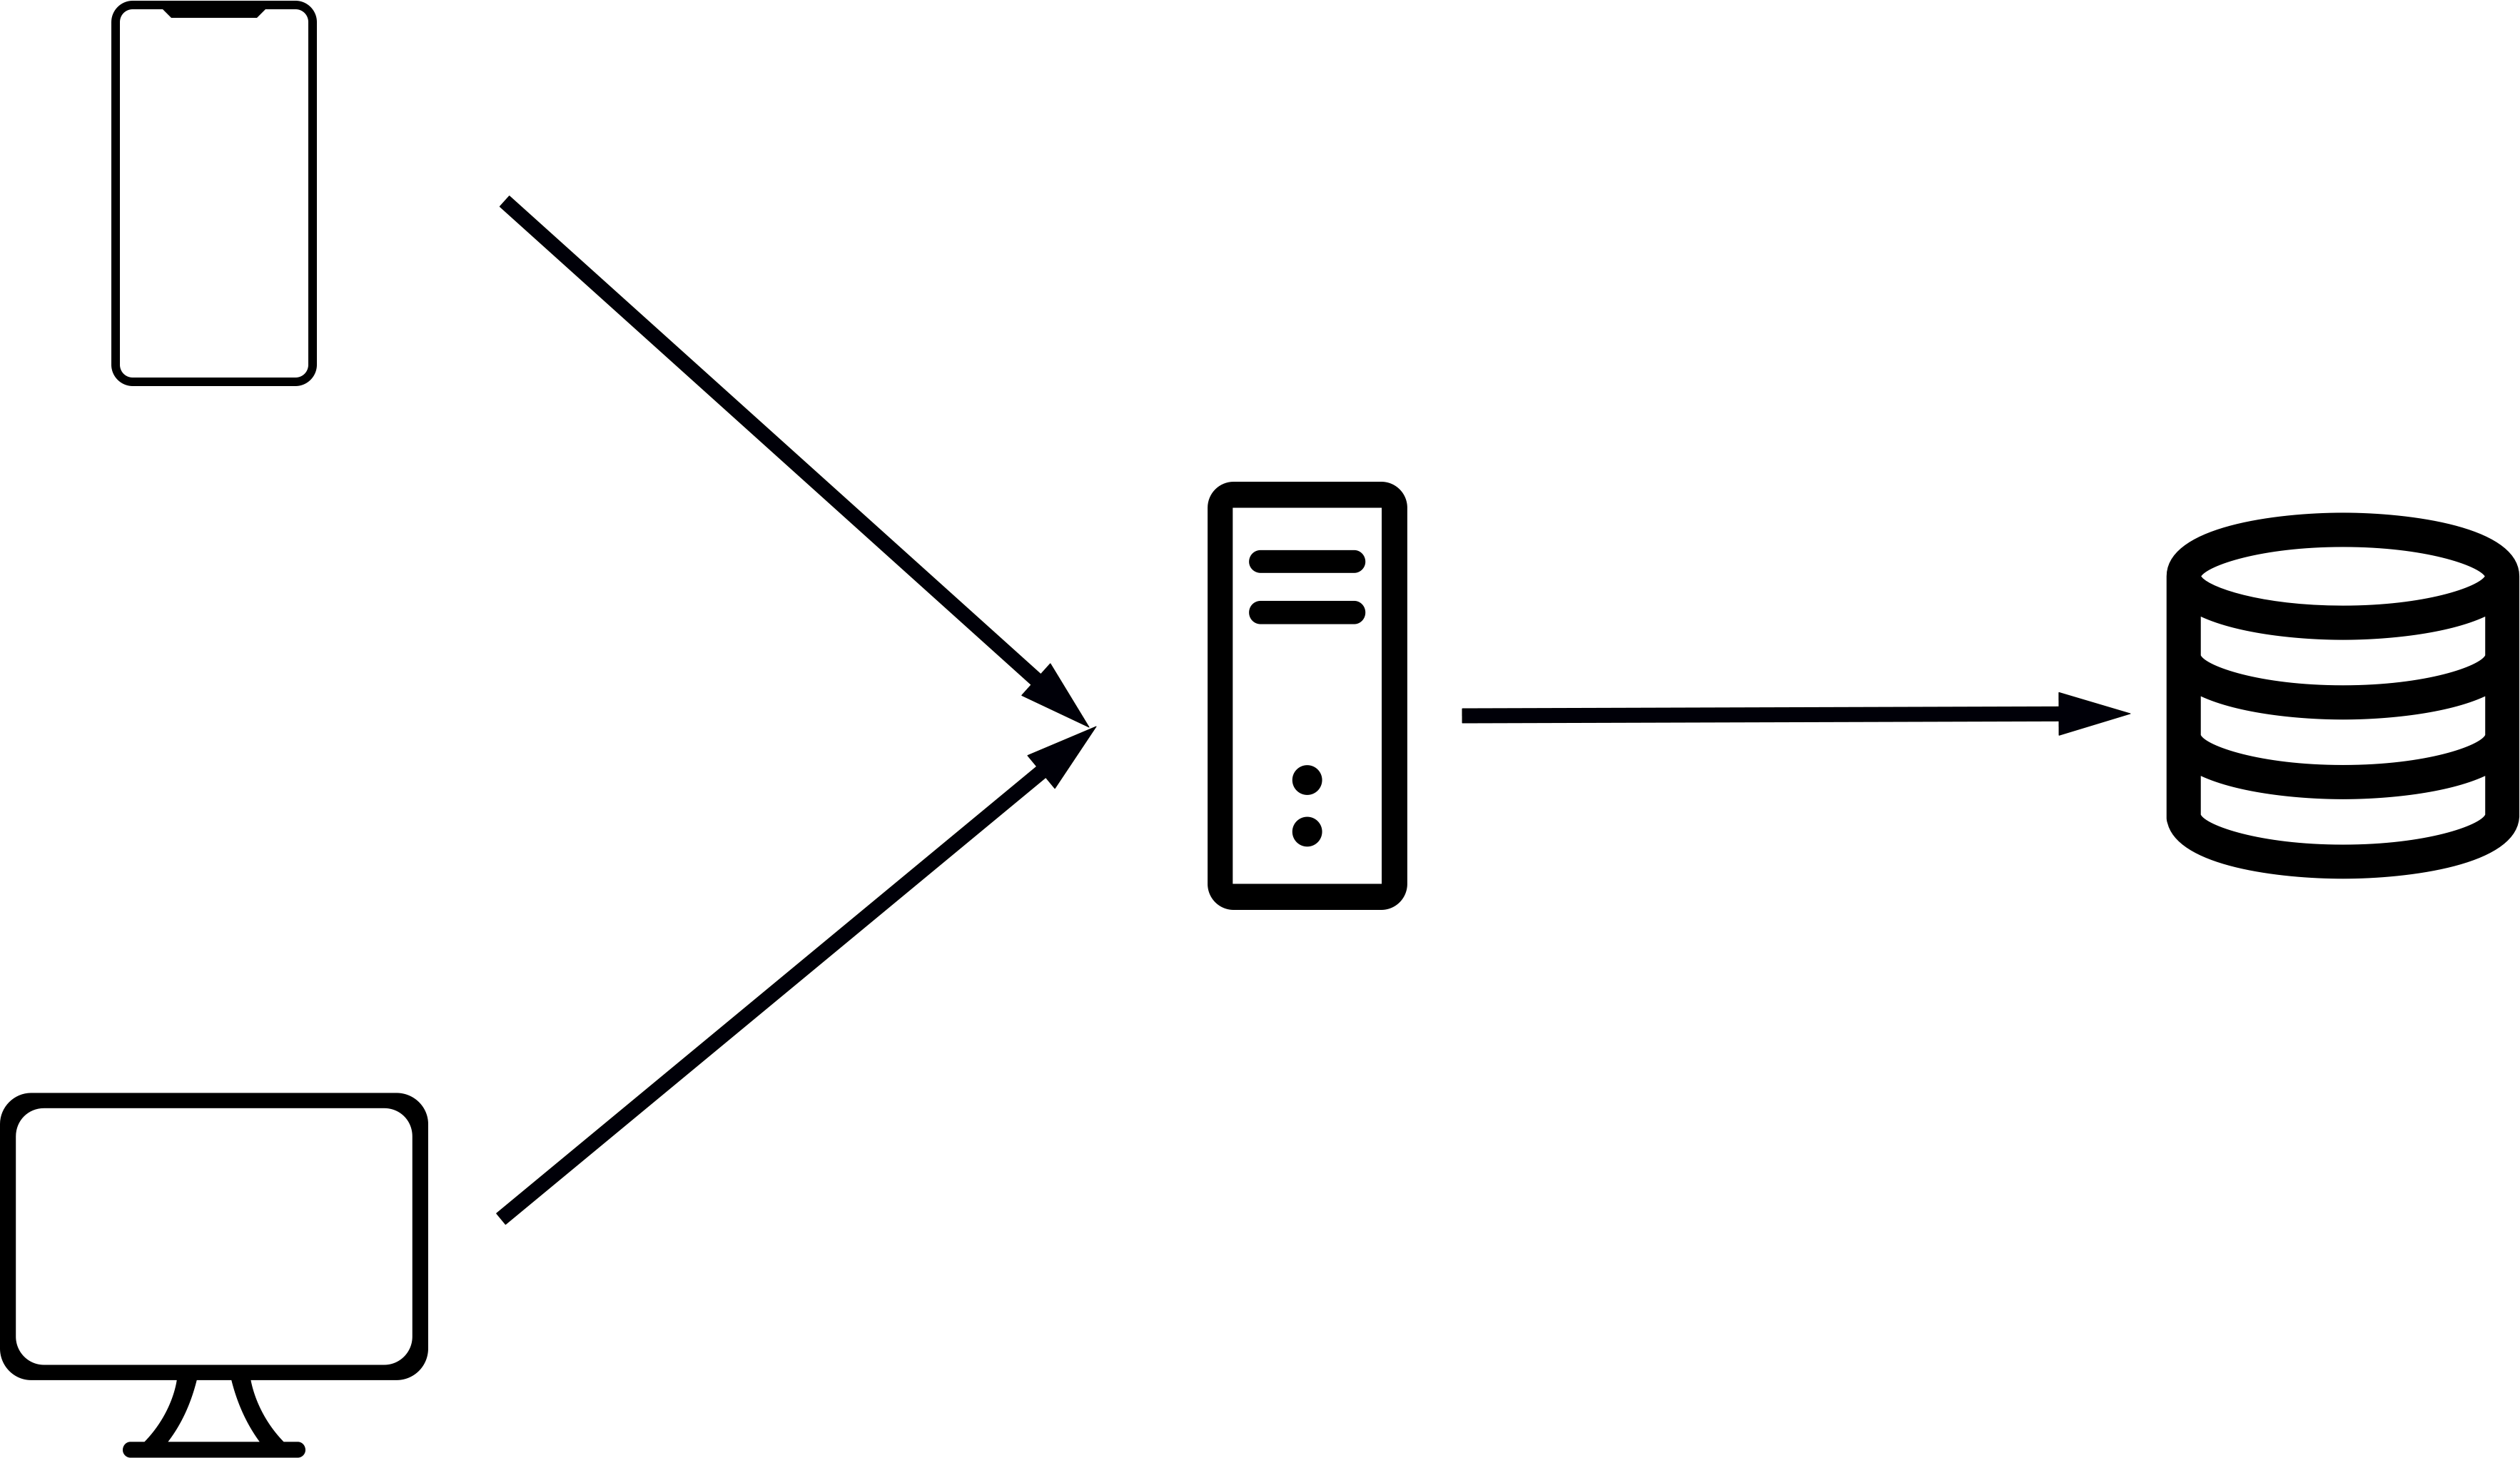
\includegraphics[scale = 0.1]{Images/AppServDb.png}
	\caption{System Overview}
\end{figure}